\chapter{\label{cha:qe_word}Extending TransQuest for Word-Level QE}

Translation quality can be estimated at different levels of granularity: word, sentence and document level \autocite{ive-etal-2018-deepquest}. So far in this thesis, we have only explored sentence-level QE \autocite{specia-etal-2020-findings-wmt}, in which QE models provide a score for each pair of source and target sentences. A more challenging task, which is currently receiving a lot of attention from the research community, is the word-level quality estimation which provides more fine-grained information about the quality of a translation, indicating which words from the source have been incorrectly translated in the target (good vs bad words), and whether the words inserted between these words are correct (good vs bad gaps). This information can be useful for post-editors by indicating the parts of a translation on which they have to focus more. Therefore, word-level QE solutions would certainly improve the efficiency of the post-editors.

Furthermore, as mentioned before, sentence-level QE models are difficult to explain as they only output a single score for the translation. The users face the difficulty of interpreting the score and how to make use of the information from the QE method. However, in contrast to that, word-level QE models provide more fine-grained information about the quality of a translation. As a result, they can improve the usability of the whole QE process. Since there is a growing interest in the NLP community for practical machine learning, we believe that having more usable QE models would improve the popularity of QE.        

With these advantages, researchers have provided many solutions for word-level QE. Similar to sentence-level QE, state-of-the-art models in word-level QE are also relying on deep learning. As we explained in Chapter \ref{cha:qe_introduction}, most of the open-source quality estimation frameworks, such as OpenKiwi, uses the same architectures for both word-level and sentence-level QE. For example, the predictor-estimator architecture used in OpenKiwi provides the best results for word-level QE too. Therefore, word-level QE also suffers from the same limitation we mentioned in the last chapter. The architectures are very complex and need a lot of computing resources to train the models, which has seriously hindered the success of word-level QE in real-world applications \autocite{ranasinghe-etal-2021-exploratory}.

To overcome this, we propose a simple architecture to perform word-level QE. The proposed architecture is very similar to the \textit{MonoTransQuest} architecture we introduced in the last chapter, which in turn was based on a state-of-the-art STS method. We only change the output layer of the \textit{MonoTransQuest} architecture so that it can produce word-level qualities. This architecture is simple and effective when compared with the current state-of-the-art word-level QE architectures such as predictor-estimator. We believe that a simpler architecture can improve the popularity of word-level QE in real-world applications. 

As mentioned in Chapter \ref{cha:qe_introduction}, word-level QE systems should have three features in them. \textit{i}. Predict the qualities of the words in the target. \textit{ii}. Predict the qualities of the words in the source. \textit{iii}. Predict the qualities of the gaps in the target. As a result, WMT word-level QE shared task has three separate evaluation metrics focussing on each of the above features. However, most of the open-source word-level QE frameworks ignore predicting the quality of the gaps in the target sentence. For example, Marmot \autocite{logacheva-etal-2016-marmot} only supports predicting the quality of the words in the target, and OpenKiwi \autocite{kepler-etal-2019-openkiwi} only supports predicting the quality of the words in the source and the target. They completely ignore predicting the quality of the gaps. Despite that, predicting the quality of the gaps in the target would be important and useful for post-editors. Therefore, when we design the proposed architecture in this chapter, we considered all three features in word-level QE; predicting the quality of the words in the target, predicting the quality of the words in the source and predicting the quality of the gaps in the target. We believe an approach that supports every feature in word-level QE will be stronger than existing solutions.

We address three research questions in this chapter:

\textbf{RQ1:} Can existing state-of-the-art STS architecture be used to predict all the features in the word-level QE task by just modifying the embeddings and output layer?

\textbf{RQ2:} Do cross-lingual embeddings have an advantage over multilingual embeddings in the word-level QE task?

\textbf{RQ3:} Can the proposed model be further improved by performing ensemble learning?

The main contributions of this chapter are as follows.
\begin{enumerate}
  \item We introduce a simple architecture to perform word-level quality estimation that predicts the quality of the words in the source sentence, target sentence and the gaps in the target sentence.
  
  \item We evaluate it on eight different language pairs in which the word-level QE data was available, and we show that the proposed architecture outperforms the current state-of-the-art word-level QE frameworks such as Marmot \autocite{logacheva-etal-2016-marmot} and OpenKiwi \autocite{kepler-etal-2019-openkiwi}.
  
  \item We suggest further improvements to the model by performing ensemble learning.
  
  \item We integrated the architecture with TransQuest, which already had two sentence-level architectures described in Chapter \ref{cha:qe_transquest}\footnote{The public GitHub repository of TransQuest is available on \url{https://github.com/tharindudr/TransQuest}}. TransQuest framework was already popular with the NLP community and adding a word-level architecture to that boosted its value. Additionally the pre-trained word-level QE models for eight language pairs are freely available to the community\footnote{Pre-trained word-level QE models are available on \url{https://huggingface.co/models?filter=microtransquest}}. 
  	
\end{enumerate}

The rest of this chapter is organised as follows. Section \ref{sec:word_level_method} discusses the methodology and the experiments conducted with eight language pairs in word-level QE.  Section \ref{sec:word_level_results} shows the results of three evaluation metrics used in word-level QE. Section \ref{sec:word_level_finetune} provides further fine-tuning strategies to improve the results. The chapter finishes with conclusions and ideas for future research directions in word-level QE.

\section{Methodology}
\label{sec:word_level_method}
The proposed architecture for the word-level QE is very similar to the \textit{MonoTransQuest} architecture in Chapter \ref{cha:qe_transquest} where the source and the target are processed through a single transformer model. The difference here is since we need quality for each word, we do not use a pooling mechanism as we did with \textit{MonoTransQuest}. Instead, we keep the state of the individual tokens to get their quality.

As we also need to consider the quality of the GAPs in word-level QE, we first add a new token to the tokeniser of the transformer called \textsc{$<$GAP$>$} which is inserted between the words in the target. We then concatenate the source and the target with a \textsc{[SEP]} token as in \textit{MonoTransQuest} architecture and feed them into a single transformer. A simple linear layer is added on top of the word and {$<$GAP$>$} embeddings to predict whether it is "Good" or "Bad" as shown in Figure \ref{fig:word_level_architecture}. Each of the softmax layers we used on top of the transformer model consists of two neurons. They provide two probabilities for each word or gap, stating the probability of being "Good" or "Bad". We consider the class with the maximum probability as the quality of a particular word or gap. As we integrated this architecture to the \textit{TransQuest} framework and it provides quality for the smallest unit possible in QE, we named the proposed word-level architecture as \textit{MicroTransQuest}. 


Similar to the sentence-level QE architectures, we used cross-lingual transformer models for this architecture. As explained in Chapter \ref{cha:qe_transquest}, XLM-R provides state-of-the-art cross-lingual transformer models. There are two pre-trained XLM-R models released by HuggingFace's Transformers library \autocite{wolf-etal-2020-transformers}; XLM-R-base and XLM-R-large. We used both of these pre-trained models in our experiments\footnote{XLM-R-large is available on \url{https://huggingface.co/xlm-roberta-large} and XLM-R-base is available on \url{https://huggingface.co/xlm-roberta-base}}. Both of these pre-trained XLM-R models cover 104 languages \autocite{conneau-etal-2020-unsupervised}, making them potentially very useful to estimate the word-level translation quality for a large number of language pairs.

\begin{figure}
	\centering
	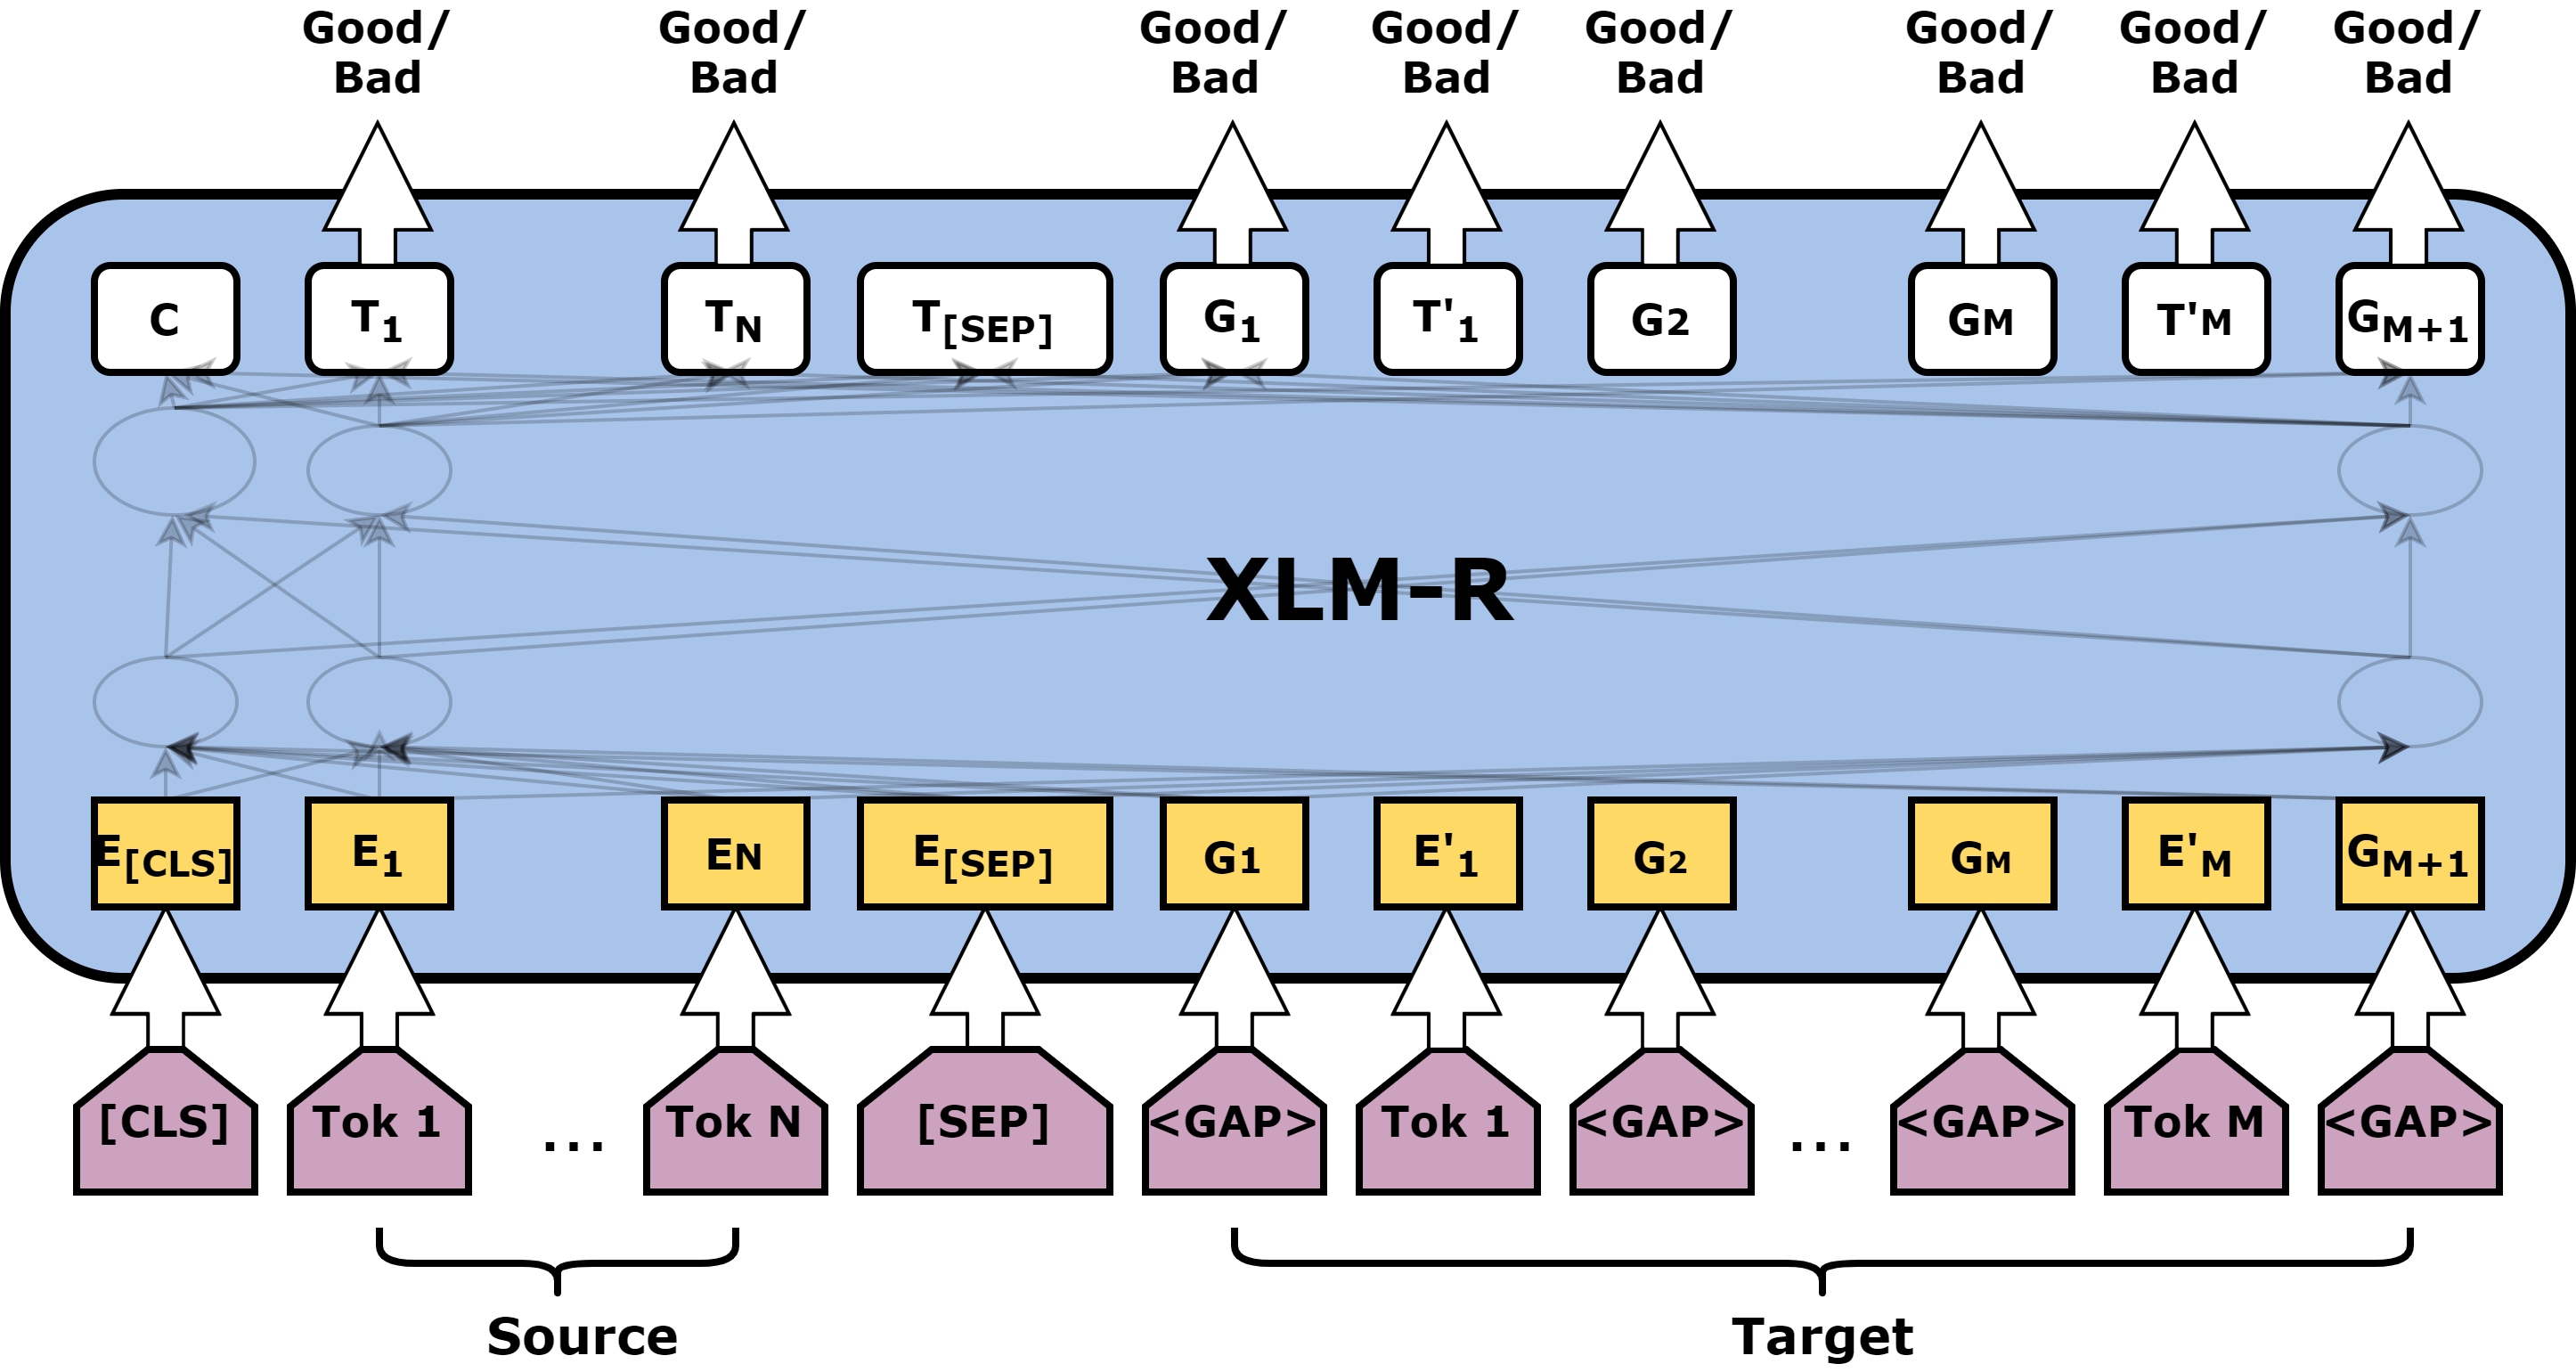
\includegraphics[scale=0.7]{figures/translation_quality_estimation/word_level/MicroTransQuest.png}
	\caption{MicroTransQuest Architecture}
	\label{fig:word_level_architecture}
\end{figure}

\subsection{Experimental Setup}
\label{sec:word_level_experiment}
We evaluated the architecture in word-level quality estimation using the data introduced in Chapter \ref{cha:qe_introduction}. We applied the same set of configurations for all the language pairs to ensure consistency between all the experiments. This also provides a good starting configuration for researchers who intend to use \textit{MicroTransQuest} on a new language pair. We used a batch-size of eight, Adam optimiser with a learning rate $1\mathrm{e}^{-5}$, and a linear learning rate warm-up over 10\% of the training data. During the training process, the parameters of the XLM-R model and the subsequent layers were updated. The models were trained using only training data. Furthermore, they were evaluated while training once in every 300 training steps using an evaluation set with one-fifth of the training data instances. We performed early stopping if the evaluation loss did not improve over ten evaluation steps. All the models were trained for three epochs.

\section{Results and Evaluation}
\label{sec:word_level_results}
For the evaluation, we used the approach proposed in the WMT shared tasks in which the classification performance is calculated using the multiplication of F1-scores ($F1_{\textit{MULTI}}$) for the `OK' and `BAD' classes against the true labels
independently: words in the target (`OK' for correct words, `BAD' for incorrect words), gaps in the target (`OK' for genuine gaps, `BAD' for gaps indicating missing words) and source words (`BAD' for words that lead to errors in the target, `OK' for other words) \autocite{specia-etal-2018-findings} as explained in Chapter \ref{cha:qe_introduction}. In WMT QE shared tasks, Word-level QE systems have been evaluated using all three of these evaluation metrics. Therefore, we follow the same process so that we can compare our results with the baselines and best systems of the respective shared task.

$F1_{\textit{MULTI}}$ for the words in the target ($F1_{\textit{MULTI}} \; Target$), $F1_{\textit{MULTI}}$ for the gaps in the target ($F1_{\textit{MULTI}} \; GAPS$) and $F1_{\textit{MULTI}}$ for the words in the source  ($F1_{\textit{MULTI}} \; Source$) are shown in Tables \ref{tab:mt_prediction}, \ref{tab:gap_prediction} and \ref{tab:source_prediction} respectively. Before WMT 2019, organisers provided separate scores for gaps and words in the target, while after WMT 2019, they produce a single result for target gaps and words. Therefore, we report ($F1_{\textit{MULTI}} \; GAPS$) only on the language pairs released in WMT 2018 in Table \ref{tab:gap_prediction}. For the language pairs in WMT 2019 and 2020, we report a single result for the target gaps and words as ($F1_{\textit{MULTI}} \; Target$) in Table \ref{tab:mt_prediction}.

\renewcommand{\arraystretch}{1.2}
\begin{table}[t]
	\begin{center}
		\small
		% \footnotesize
		\scalebox{0.8}{
			\begin{tabular}{l l  c c c c c c c c} 
				%\hline
				\toprule
				& & \multicolumn{4}{c}{\bf Mid-resource} & \multicolumn{4}{c}{\bf High-resource}\\\cmidrule(r){3-6}\cmidrule(r){7-10}
				&{\bf Method} & \makecell{En-Cs \\ SMT} & \makecell{ En-Ru \\ NMT} & \makecell{En-Lv \\ SMT} & \makecell{En-Lv \\ NMT} & \makecell{De-En \\ SMT} & \makecell{En-Zh \\ NMT} & \makecell{En-De \\ SMT } & \makecell{En-De \\ NMT} \\
				\midrule
				\multirow{1}{*}{\bf I} & MicroTransQuest & 0.6081 & 0.5592 & 0.5939 & 0.5868 & 0.6485 & 0.5602 & 0.6348 & 0.5013\\
				\midrule
				\multirow{1}{*}{\bf II} & MicroTransQuest-base & 0.5642 & 0.5132 & 0.5579 & 0.5431 & 0.6001 & 0.5202 & 0.5985 & 0.4698 \\
				\midrule
				\multirow{1}{*}{\bf III} & MicroTransQuest $\otimes$ & \textbf{0.6154} & \textbf{0.5672} & \textbf{0.6123} & \textbf{0.6003} & \textbf{0.6668} & 0.5678 & \textbf{0.6451} & 0.5121 \\
				\midrule
				\multirow{3}{*}{\bf IV} & Marmot & 0.4449 & NR & 0.3445 & 0.4208 & 0.4373 & NR & 0.3653 & NR \\
				& OpenKiwi & NR & 0.2412 & NR & NR & NR & 0.5583 & NR & 0.4111 \\
				& Best system & 0.4449 & 0.4780 & 0.3618 & 0.4293 & 0.6012 & \textbf{0.6415} & 0.6246 &  \textbf{0.6186} \\
				\midrule
				\multirow{1}{*}{\bf V} & MicroTransQuest-B & 0.5462 & 0.4987 & 0.5043 & 0.5132 & 0.5643 & 0.4892 & 0.5381 & 0.4371 \\
				\bottomrule
				%\bottomrule
			\end{tabular}
		}
	\end{center}
	\caption[$F1_{\textit{MULTI}} \; Target$ between the algorithm predictions and human annotations]{$F1_{\textit{MULTI}} \; Target$ between the algorithm predictions and human annotations. The best result for each language by any method is highlighted in bold. Row \textbf{I} shows the results for XLM-R-large model and Row \textbf{II} shows the results for XLM-R-base. Row \textbf{III} presents the results for further fine-tuning strategies explained in Section \ref{sec:word_level_finetune}. Row \textbf{IV} shows the results of the baseline methods and the best system submitted for the language pair in that competition. \textbf{NR} implies that a particular result was \textit{not reported} by the organisers. Row \textbf{V} presents the results of the multilingual BERT (mBERT) model in \textit{MicroTransQuest}.} 
	\label{tab:mt_prediction}
\end{table}


\renewcommand{\arraystretch}{1.2}
\begin{table}[t]
	\begin{center}
	\small
	% \footnotesize
	\scalebox{1.0}{
		\begin{tabular}{l l  c c c c c } 
			%\hline
			\toprule
			& & \multicolumn{3}{c}{\bf Mid-resource} & \multicolumn{2}{c}{\bf High-resource}\\\cmidrule(r){3-5}\cmidrule(r){6-7}
			&{\bf Method} & \makecell{En-Cs \\ SMT} & \makecell{En-Lv \\ SMT} & \makecell{En-Lv \\ NMT} & \makecell{De-En \\ SMT}  & \makecell{En-De \\ SMT }  \\
			\midrule
			\multirow{1}{*}{\bf I} & MicroTransQuest & 0.2018 & 0.2356 & 0.1664 & 0.4203 & 0.4927 \\
			\midrule
			\multirow{1}{*}{\bf II} & MicroTransQuest-base & 0.1876 & 0.2132 & 0.1452 & 0.4098 & 0.4679 \\
			\midrule
			\multirow{1}{*}{\bf III} & MicroTransQuest $\otimes$ & \textbf{0.2145} & \textbf{0.2437} & \textbf{0.1764} & \textbf{0.4379} & \textbf{0.4982} \\
			\midrule
			\multirow{2}{*}{\bf IV} & Marmot & NS & NS & NS & NS & NS   \\
			& Best system & 0.1671 & 0.1386 & 0.1598 & 0.3176 & 0.3161  \\
			\midrule
			\multirow{1}{*}{\bf V} & MicroTransQuest-B & 0.1778 & 0.2089 & 0.1387 & 0.3892 & 0.4371  \\
			\bottomrule
			%\bottomrule
		\end{tabular}
	}
\end{center}
	\caption[$F1_{\textit{MULTI}} \; GAPS$ between the algorithm predictions and human annotations]{$F1_{\textit{MULTI}} \; GAPS$ between the algorithm predictions and human annotations. The best result for each language by any method is highlighted in bold. Row \textbf{I} shows the results for XLM-R-large model and Row \textbf{II} shows the results for XLM-R-base. Row \textbf{III} presents the results for further fine-tuning strategies explained in Section \ref{sec:word_level_finetune}. Row \textbf{IV} shows the results of the baseline methods and the best system submitted for the language pair in that competition. \textbf{NS} implies that a particular baseline does \textit{not support} predicting quality of gaps. Row \textbf{V} presents the results of the multilingual BERT (mBERT) model in \textit{MicroTransQuest}.} 
	\label{tab:gap_prediction}
\end{table}


\renewcommand{\arraystretch}{1.2}
\begin{table}[t]
	\begin{center}
		\small
		% \footnotesize
		\scalebox{0.8}{
			\begin{tabular}{l l  c c c c c c c c} 
				%\hline
				\toprule
				& & \multicolumn{4}{c}{\bf Mid-resource} & \multicolumn{4}{c}{\bf High-resource}\\\cmidrule(r){3-6}\cmidrule(r){7-10}
				&{\bf Method} & \makecell{En-Cs \\ SMT} & \makecell{ En-Ru \\ NMT} & \makecell{En-Lv \\ SMT} & \makecell{En-Lv \\ NMT} & \makecell{De-En \\ SMT} & \makecell{En-Zh \\ NMT} & \makecell{En-De \\ SMT } & \makecell{En-De \\ NMT} \\
				\midrule
				\multirow{1}{*}{\bf I} & MicroTransQuest & 0.5327 & 0.5543 & 0.4945 & 0.4880 & 0.4824 & 0.4040 & 0.5269 & 0.4456\\
				\midrule
				\multirow{1}{*}{\bf II} & MicroTransQuest-base & 0.5134 & 0.5287 & 0.4652 & 0.4571 & 0.4509 & 0.3876 & 0.5012 & 0.4185 \\
				\midrule
				\multirow{1}{*}{\bf III} & MicroTransQuest $\otimes$ & \textbf{0.5431} & \textbf{0.5640} & \textbf{0.5076} & \textbf{0.4892} & \textbf{0.4965} & 0.4145 & \textbf{0.5387} & 0.4578 \\
				\midrule
				\multirow{3}{*}{\bf IV} & Marmot & NS & NR & NS & NS & NS & NR & NS & NR \\
				& OpenKiwi & NR & 0.2647 & NR & NR & NR & 0.3729 & NR & 0.3717 \\
				& Best system & 0.3937 & 0.4541 & 0.4945 & 0.3614 & 0.3200 & \textbf{0.4462} & 0.3368 &  \textbf{0.5672} \\
				\midrule
				\multirow{1}{*}{\bf V} & MicroTransQuest-B & 0.4987 & 0.5098 & 0.4441 & 0.4256 & 0.4187 & 0.3567 & 0.4672 & 0.3985 \\
				\bottomrule
				%\bottomrule
			\end{tabular}
		}
	\end{center}
	\caption[$F1_{\textit{MULTI}} \; Source$ between the algorithm predictions and human annotations]{$F1_{\textit{MULTI}} \; Source$ between the algorithm predictions and human annotations. The best result for each language by any method is highlighted in bold. Row \textbf{I} shows the results for XLM-R-large model and Row \textbf{II} shows the results for XLM-R-base. Row \textbf{III} presents the results for further fine-tuning strategies explained in Section \ref{sec:word_level_finetune}. Row \textbf{IV} shows the results of the baseline methods and the best system submitted for the language pair in that competition. \textbf{NR} implies that a particular result was \textit{not reported} by the organisers. Row \textbf{V} presents the results of the multilingual BERT (mBERT) model in \textit{MicroTransQuest}.} 
	\label{tab:source_prediction}
\end{table}

Raw I in Tables \ref{tab:mt_prediction}, \ref{tab:gap_prediction} and \ref{tab:source_prediction} shows the results for \textit{MicroTransQuest} with XLM-R-large and Raw II in Tables  \ref{tab:mt_prediction}, \ref{tab:gap_prediction} and \ref{tab:source_prediction} shows the results for \textit{MicroTransQuest} with XLM-R-base. As can be seen in results, XLM-R-large always outperformed XLM-R-base. Therefore, we use the results we got from XLM-R-large for the following analysis.
 
In $F1_{\textit{MULTI}} \; Target$ evaluation metric in word-level QE, as shown in Table \ref{tab:mt_prediction}, \textit{MicroTransQuest} outperforms OpenKiwi and Marmot in all the language pairs we experimented. Additionally, \textit{MicroTransQuest} achieves $\approx$ 0.3 $F1_{\textit{MULTI}}$ score boost over OpenKiwi in the En-Ru NMT. Furthermore, \textit{MicroTransQuest} gained $\approx$ 0.15-0.2 $F1_{\textit{MULTI}}$ score boost over Marmot in all the language pairs. Table \ref{tab:mt_prediction}  also gives the results of the best system submitted for a particular language pair. It is worth noting that the \textit{MicroTransQuest} results surpass the best system in all the language pairs, with the exception of the En-De NMT and En-Zh NMT datasets.
 
 In $F1_{\textit{MULTI}} \; GAPS$ evaluation metric in word-level QE, as shown in Table \ref{tab:gap_prediction} \textit{MicroTransQuest} outperforms best systems submitted to the respective shared tasks in all the language pairs we experimented. \textit{MicroTransQuest} achieves $\approx$ 0.05-0.2 $F1_{\textit{MULTI}}$ score boost over best systems. Notably, \textit{MicroTransQuest} achieves $\approx$ 0.2 $F1_{\textit{MULTI}}$ score boost over the best system in En-De SMT. As we mentioned before, it should be noted that neither of the baselines, Marmot, nor OpenKiwi supports predicting the quality of \textit{gaps} in the target sentence. Since \textit{MicroTransQuest} supports this and produces state-of-the-results in this evaluation metric, we believe that using \textit{MicroTransQuest} in word-level QE would be beneficial than using OpenKiwi and Marmot.
 
Finally, in $F1_{\textit{MULTI}} \; Source$ evaluation metric, as shown in Table \ref{tab:source_prediction} \textit{MicroTransQuest} outperforms OpenKiwi in all the language pairs we experimented. It should be noted that Marmot does not support predicting the quality of the words in the source. On the other hand, OpenKiwi supports this, but \textit{MicroTransQuest} achieves $\approx$ 0.05-0.3 $F1_{\textit{MULTI}}$ score boost in all the language pairs. Furthermore, \textit{MicroTransQuest} results surpass the best system in all the language pairs with the exception of the En-De NMT and En-Zh NMT datasets.

With these results, we can answer our \textbf{RQ1:} \textit{Can existing state-of-the-art STS architecture be used to predict all features in the word-level QE task by just modifying the embeddings and the output layer?} We show that the state-of-the-art STS method based on cross-lingual transformer models can be used in word-level QE  by changing the output layer. It outperforms current state-of-the-art word-level QE methods such as OpenKiwi that relies on complex neural network architectures. Our proposed architecture is not only simple, but also achieves state-of-the-art results in all the language pairs we experimented. Furthermore, \textit{MicroTransQuest} is the only architecture that supports predicting the quality of the gaps in target. We believe that the way we designed the architecture based on state-of-the-art STS architectures gave us the ability to support predicting the quality of the gaps in target with \textit{MicroTransQuest}.

Row VI in Tables \ref{tab:mt_prediction}, \ref{tab:gap_prediction} and \ref{tab:source_prediction} shows the results of multilingual BERT (mBERT) in \textit{MicroTransQuest} architecture. We used the same settings similar to XLM-R. The results show that the XLM-R model outperforms the mBERT model in all the language pairs. As shown in Row II in Tables \ref{tab:mt_prediction}, \ref{tab:gap_prediction} and \ref{tab:source_prediction} even XLM-R-base model outperform mBERT model in all the languages pairs. Therefore, we can safely assume that the cross-lingual nature of the XLM-R transformers had a clear impact on the results. This observation is similar to what we experienced in Chapter \ref{cha:qe_transquest} with sentence-level QE experiments.

With this, we can answer our \textbf{RQ2:} Using cross-lingual embeddings with STS architecture proved advantageous rather than using multilingual embeddings. As far as we know, this is the first time XLM-R was used in a task related to detecting missing words. With the results we got from predicting the quality of the gaps in target, we show that XLM-R can be used in tasks similar to detecting missing words.
 

\section{Further Improvements}
\label{sec:word_level_finetune}
In this section, we improve the results of \textit{MicroTransQuest} through ensemble learning as we did with sentence-level quality estimation. As mentioned before in Section \ref{sec:word_level_method} softmax layer provides two probabilities for each word or gap. We calculated these probabilities for each word using XLM-R-large and XLM-R base. Then we performed a weighted average ensemble on these probabilities, and we consider the class with the highest probability after performing the ensemble as the quality of the word or gap. We experimented on weights 0.8:0.2, 0.6:0.4, 0.5:0.5 on the output of XLM-R-large and output from XLM-R-base, respectively. Since the results we got from XLM-R-base transformer model are slightly worse than the results we got from XLM-R-large we did not consider the weight combinations that gives higher weight to XLM-R-base transformer model results. We obtained the best results when we used the weights 0.6:0.4. We report the results from this step in Row III of Tables \ref{tab:mt_prediction}, \ref{tab:gap_prediction} and \ref{tab:source_prediction} as MicroTransQuest $\otimes$.

As shown in Tables \ref{tab:mt_prediction}, \ref{tab:gap_prediction} and \ref{tab:source_prediction} ensemble learning improved the results for \textit{MicroTransQuest} in all three evaluation metrics. For all the language pairs $F1_{\textit{MULTI}} \; Target$, $F1_{\textit{MULTI}} \; GAPS$, and $F1_{\textit{MULTI}} \; Source$ scores gained $\approx$ 0.01-0.02 boost with ensemble learning. This answers our \textbf{RQ3:} \textit{Can the proposed model be further improved by performing ensemble learning?} We show that ensemble learning can be used to improve the word-level QE results similar to sentence-level QE. In fact, ensemble learning provided the best results for \textit{MicroTransQuest} in all the language pairs we experimented.

\section{Conclusion}
In this chapter, we explored word-level QE with transformers. We introduced a new architecture based on transformers to perform word-level QE. The proposed architecture is very similar to the sentence-level QE architecture; \textit{MonoTransQuest}. However, the output layers are different to \textit{MonoTransQuest} so that they keep the state of the individual tokens to get their quality. We evaluated the proposed architecture; \textit{MicroTransQuest} on eight language pairs where the word-level QE data was available.  It outperforms other open-source tools like OpenKiwi and Marmot on all three evaluations metrics of word-level quality estimation and yields new state-of-the-art word-level QE results. Furthermore, \textit{MicroTransQuest} is the only open-source architecture that supports predicting the quality of the gaps in the target sentence. The architecture we proposed in this chapter is very simple compared to the predictor-estimator architecture in OpenKiwi, yet this architecture produces better results. We further improved the results with ensemble learning showed that \textit{MicroTransQuest} outperforms the majority of the best systems submitted for that language in each shared task. We can conclude that state-of-the-art STS architecture can also be used in word-level QE by doing small modifications to the output layers.

The implementation of the architecture, which is based on PyTorch \autocite{NEURIPS2019_9015} and Hugging Face \autocite{wolf-etal-2020-transformers}, has been integrated into the TransQuest framework \autocite{ranasinghe-etal-2020-transquest} which won the WMT 2020 QE task \autocite{specia-etal-2020-findings-wmt} on sentence-level direct assessment \autocite{ranasinghe-etal-2020-transquest-wmt2020}\footnote{The details about the word-level QE architecture in TransQuest is available on \url{http://tharindu.co.uk/TransQuest/architectures/word_level_architecture/}}. The pre-trained word-level QE models for eight language pairs are available to the public on HuggingFace model hub. 

One limitation of the proposed architecture is that it only predicts word-level qualities. Managing two models to predict the word-level and sentence-level qualities separately would be chaotic in some situations as the two models can produce contradictory predictions. Therefore, in the future, we hope to explore multi-task learning for word-level and sentence-level QE \autocite{Caruana1997}. The two tasks are related as word-level quality contributes to the sentence-level quality in general. Therefore we believe that a multi-task architecture that can learn both tasks simultaneously can be advantageous. 

As discussed at multiple points in this thesis, pre-trained models based on transformers are big in size. Therefore, managing several of them for each language pair would be chaotic in a real-world application for word-level QE. As a solution for that, we explore multilingual word-level QE models in Chapter \ref{cha:qe_multilingual} in Part III of the thesis.



